%/*
% * SPDX-FileCopyrightText: 2021 Stefan Begerad <stefan@begerad.de>
% *
% * SPDX-License-Identifier: GPL-3.0-or-later
% */

\begin{frame}
  \frametitle{Datenaufkommen über Mobilfunk}
  Dede Bordrechner und Dede Server tauschen Daten per Mobilfunk aus.
  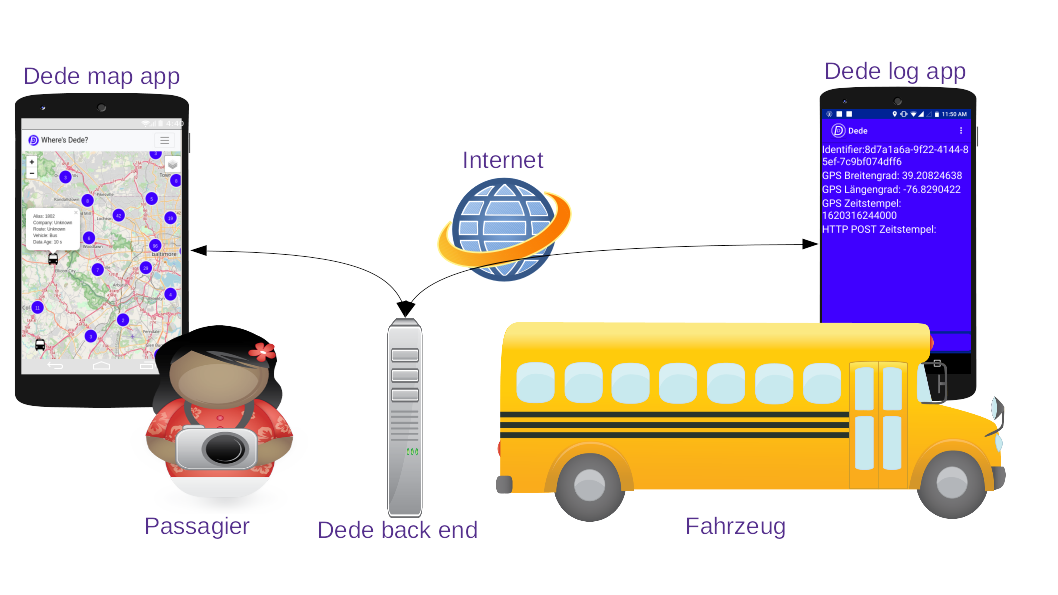
\includegraphics[width=\paperwidth]{dede/dede-concept}
\end{frame}

\begin{frame}
  \frametitle{Datenaufkommen: Protokolle}
  \begin{itemize}
  \item Internet-typischer Protokollstapel: IP, TCP, HTTP
  \item HTTP folgt dem Anfrage/Anwort-Schema
  \item HTTP wird typischer Weise um Authentifizierung und Verschlüsserlung erweitert (HTTPS)
  \end{itemize}
  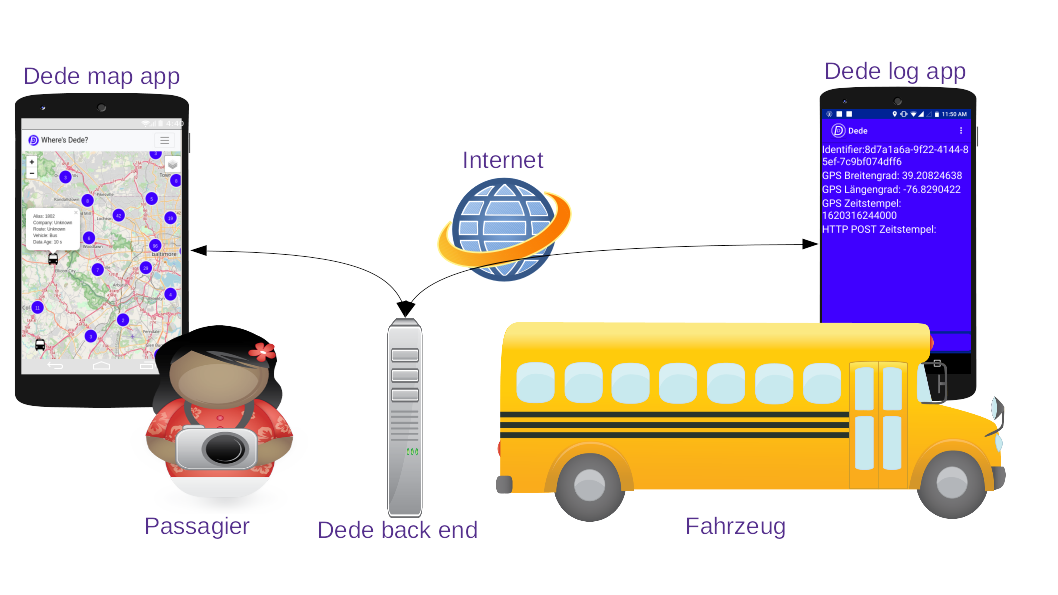
\includegraphics[width=0.5\paperwidth]{dede/dede-concept}
\end{frame}

\begin{frame}
  \frametitle{Datenaufkommen über Mobilfunk: HTTP vs. HTTPS}
  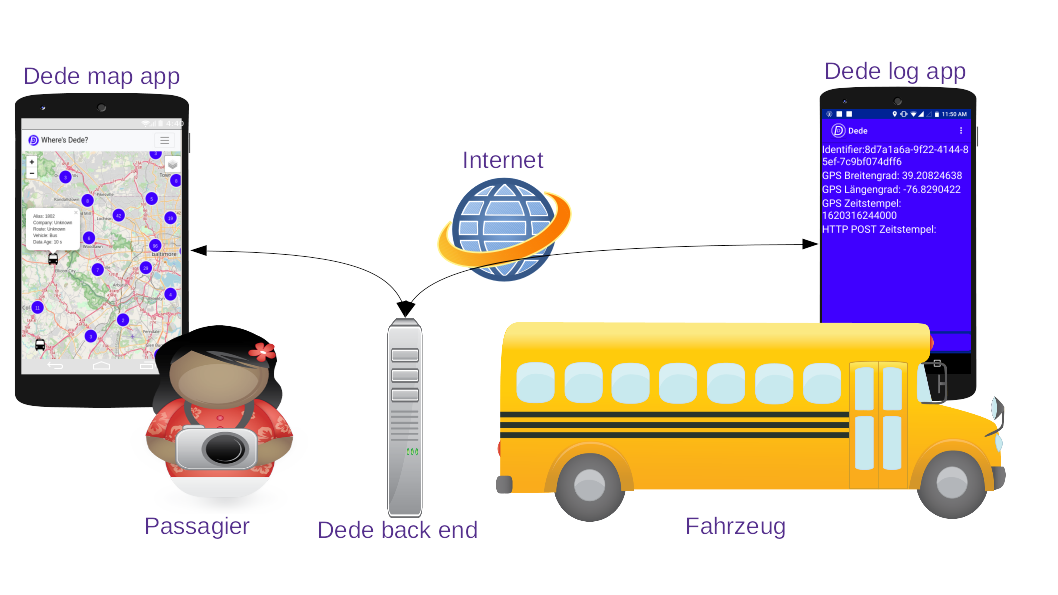
\includegraphics[width=0.7\paperwidth]{dede/dede-concept}
  \begin{tabular}{lcccc}
    Datenaufkommen   & HTTP  & HTTPS \\\hline
    pro Minute in KB & 1,24  & 1,3   \pause\\
    pro Stunde in KB & 74,34 & 78,06 \pause\\
    pro Tag in MB    & 1,78  & 1,87 \pause\\
    pro Monat in MB  & 55,31 & 58,08 \pause\\
    pro Jahr in MB   & 651,22& 683,81
  \end{tabular}
\end{frame}

\begin{frame}
  \frametitle{Datenaufkommen über Mobilfunk: HTTP}
  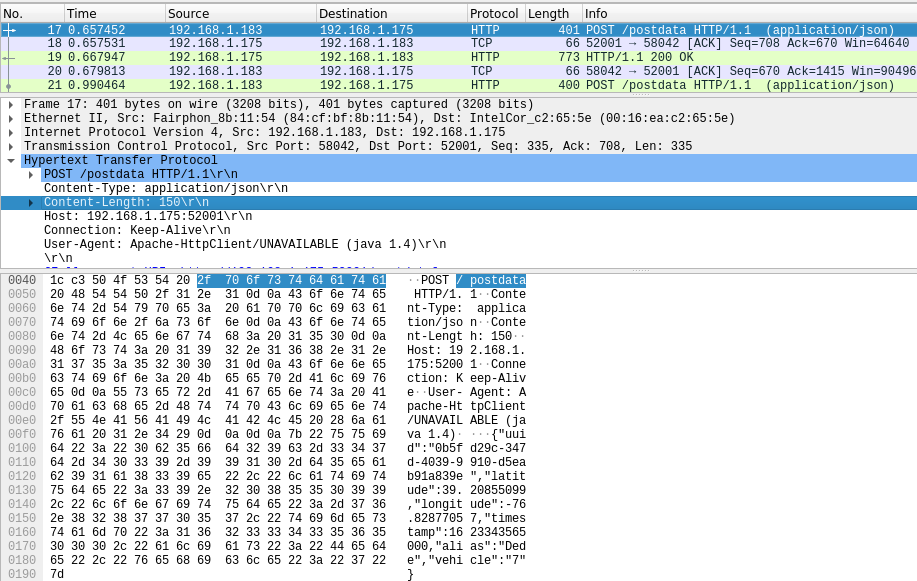
\includegraphics[width=0.88\paperwidth]{dede/dede-obc-wireshark-http-post}
\end{frame}

\begin{frame}
  \frametitle{Datenaufkommen über Mobilfunk: HTTP}
  \begin{itemize}
  \item Pro Positionserfassung erstellt der Dede Bordrechner ein Datenobjekt in einer Größe von 150 Byte.
  \item Der Dede Bordrechner sendet eine HTTP POST-Anfrage in einer Größe von 401 Byte.
  \item Es resultiert ein Datenaufkommen von 1239 Byte pro Positionserfassung.
  \end{itemize}
  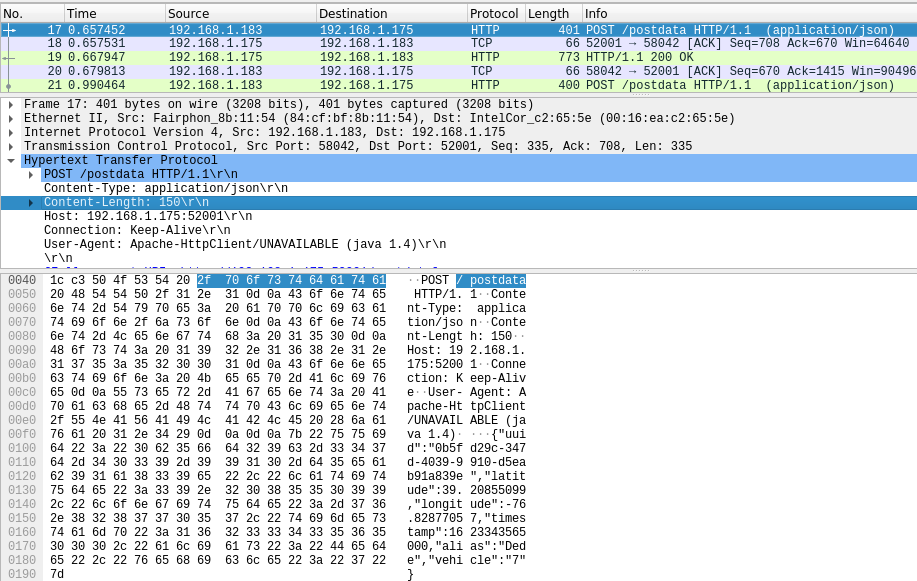
\includegraphics[width=0.5\paperwidth]{dede/dede-obc-wireshark-http-post}
\end{frame}

\begin{frame}
  \frametitle{Datenaufkommen über Mobilfunk: HTTP}
  Annahme: Der Dede Bordrechner erfasst die Position einmal pro Minute.
  \begin{itemize}
  \item Datenaufkommen pro Minute: 1239 Byte/ 1,24 KB
  \item Datenaufkommen pro Stunde: 74,34 KB
  \item Datenaufkommen pro Tag: 1,78 MB
  \item Datenaufkommen pro Monat: 55,31 MB
  \item Datenaufkommen pro Jahr: 651,22 MB
  \end{itemize}
  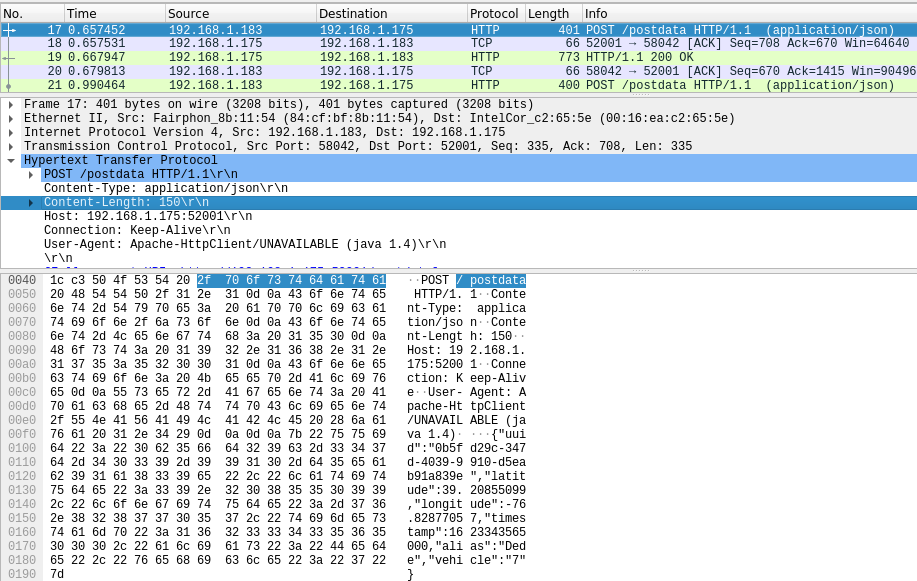
\includegraphics[width=0.5\paperwidth]{dede/dede-obc-wireshark-http-post}
\end{frame}

\begin{frame}
  \frametitle{Datenaufkommen über Mobilfunk: HTTPS}
  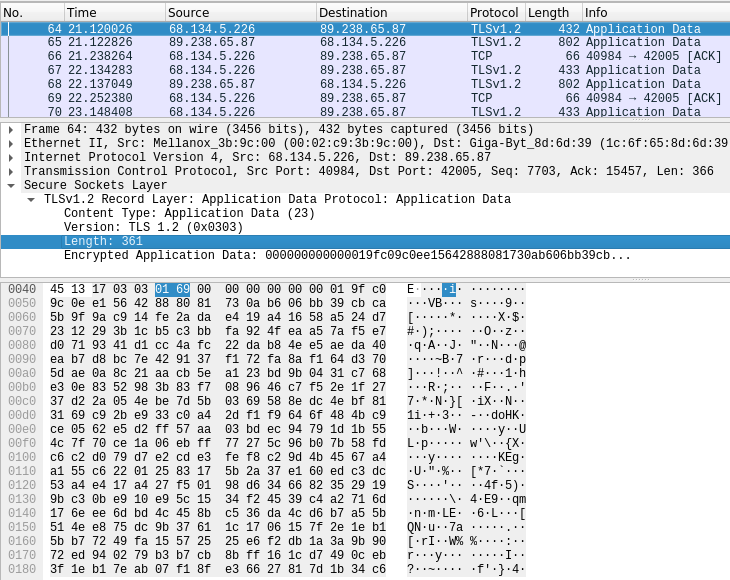
\includegraphics[width=0.80\paperwidth]{dede/dede-obc-wireshark-https-post}
\end{frame}

\begin{frame}
  \frametitle{Datenaufkommen über Mobilfunk: HTTPS}
  \begin{itemize}
  \item Pro Positionserfassung erstellt der Dede Bordrechner ein Datenobjekt in einer Größe von 150 Byte.
  \item Der Dede Bordrechner sendet eine HTTPS POST-Anfrage in einer Größe von 433 Byte.
  \item Es resultiert ein Datenaufkommen von 1301 Byte pro Positionserfassung.
  \end{itemize}
  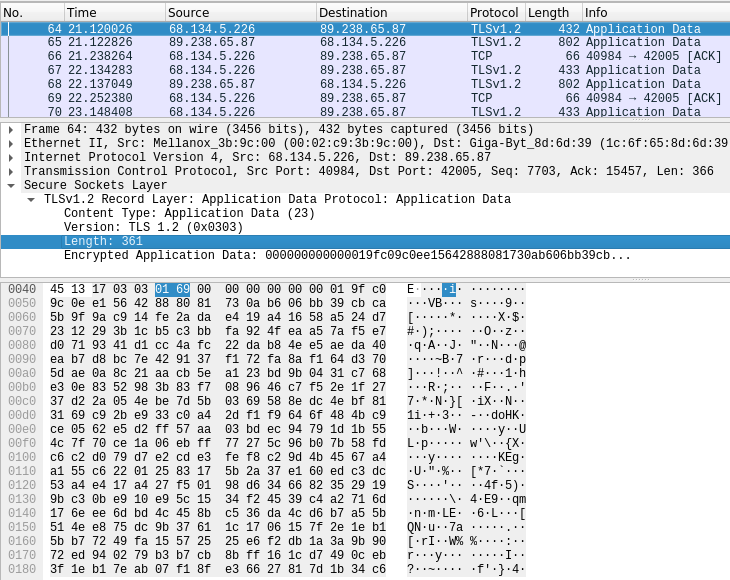
\includegraphics[width=0.5\paperwidth]{dede/dede-obc-wireshark-https-post}
\end{frame}

\begin{frame}
  \frametitle{Datenaufkommen über Mobilfunk: HTTPS}
  Annahme: Der Dede Bordrechner erfasst die Position einmal pro Minute.
  \begin{itemize}
  \item Datenaufkommen pro Minute: 1301 Byte/ 1,3 KB
  \item Datenaufkommen pro Stunde: 78,06 KB
  \item Datenaufkommen pro Tag: 1,87 MB
  \item Datenaufkommen pro Monat: 58,08 MB
  \item Datenaufkommen pro Jahr: 683,81 MB
  \end{itemize}
  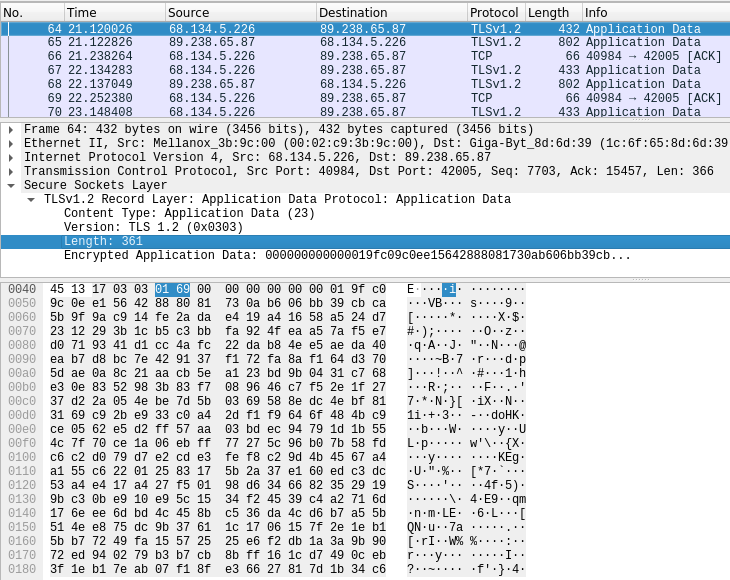
\includegraphics[width=0.5\paperwidth]{dede/dede-obc-wireshark-https-post}
\end{frame}
